%%%%%%%%%%%%%%%%%%%%%%%%%%%%%%%%%%%%%%%%%%%%%%%%%%%%%%%%%%%%
%%  Class 1, NE 155
%%

\documentclass[xcolor=x11names,compress]{beamer}

\definecolor{CoolBlack}{rgb}{0.0, 0.18, 0.39}
%% General document %%%%%%%%%%%%%%%%%%%%%%%%%%%%%%%%%%
\usepackage{graphicx}
\usepackage{tikz}
\usetikzlibrary{decorations.fractals}
\usepackage{hyperref}
%%%%%%%%%%%%%%%%%%%%%%%%%%%%%%%%%%%%%%%%%%%%%%%%%%%%%%

%% Beamer Layout %%%%%%%%%%%%%%%%%%%%%%%%%%%%%%%%%%
\useoutertheme[subsection=false,shadow]{miniframes}
\useinnertheme{default}
\usefonttheme{serif}
\usepackage{palatino}
\usepackage{tabu}
% Links
\usepackage{hyperref}
\definecolor{links}{HTML}{003262}
\hypersetup{colorlinks,linkcolor=,urlcolor=links}

% addition of color
\usepackage{xcolor}
\definecolor{CoolBlack}{rgb}{0.0, 0.18, 0.39}
\definecolor{byellow}{rgb}{0.55037, 0.38821, 0.06142}
\definecolor{dgreen}{rgb}{0.,0.6,0.}
\definecolor{RawSienna}{cmyk}{0,0.72,1,0.45}
\definecolor{forestgreen(web)}{rgb}{0.13, 0.55, 0.13}
\definecolor{cardinal}{rgb}{0.77, 0.12, 0.23}

\setbeamerfont{title like}{shape=\scshape}
\setbeamerfont{frametitle}{shape=\scshape}

\setbeamercolor*{lower separation line head}{bg=CoolBlack}
\setbeamercolor*{normal text}{fg=black,bg=white}
\setbeamercolor*{alerted text}{fg=dgreen} % just testing; I think this looks better
\setbeamercolor*{example text}{fg=black}
\setbeamercolor*{structure}{fg=black}

\setbeamercolor*{palette tertiary}{fg=black,bg=black!10}
\setbeamercolor*{palette quaternary}{fg=black,bg=black!10}

% Margins
\usepackage{changepage}

\mode<presentation>
{
  \definecolor{berkeleyblue}{HTML}{003262}
  \definecolor{berkeleygold}{HTML}{FDB515}
  \usetheme{Boadilla}      % or try Darmstadt, Madrid, Warsaw, Boadilla...
  %\usecolortheme{dove} % or try albatross, beaver, crane, ...
  \setbeamercolor{structure}{fg=berkeleyblue,bg=berkeleygold}
  \setbeamercolor{palette primary}{bg=berkeleyblue,fg=white} % changed this
  \setbeamercolor{palette secondary}{fg=berkeleyblue,bg=berkeleygold} % changed this
  \setbeamercolor{palette tertiary}{bg=berkeleyblue,fg=white} % changed this
  \usefonttheme{structurebold}  % or try serif, structurebold, ...
  \useinnertheme{circles}
  \setbeamertemplate{navigation symbols}{}
  \setbeamertemplate{caption}[numbered]
  \usebackgroundtemplate{}
}
%---

\renewcommand{\(}{\begin{columns}}
\renewcommand{\)}{\end{columns}}
\newcommand{\<}[1]{\begin{column}{#1}}
\renewcommand{\>}{\end{column}}

% adding slide numbers
\addtobeamertemplate{navigation symbols}{}{%
    \usebeamerfont{footline}%
    \usebeamercolor[fg]{footline}%
    \hspace{1em}%
    \insertframenumber/\inserttotalframenumber
}

% equation stuff
\newcommand{\Macro}{\ensuremath{\Sigma}}
\newcommand{\Sn}{\ensuremath{S_N} }
\newcommand{\vOmega}{\ensuremath{\hat{\Omega}}}
\usepackage{mathrsfs}
\usepackage[mathcal]{euscript}
\usepackage{amssymb}
\usepackage{amsthm}
\usepackage{epsfig}
\usepackage{amsmath}
%%%%%%%%%%%%%%%%%%%%%%%%%%%%%%%%%%%%%%%%%%%%%%%%%%
% title stuff for footer
\title{NE 155}
\author{R.\ N.\ Slaybaugh}
\date{January 20, 2016}

\begin{document}

%%%%%%%%%%%%%%%%%%%%%%%%%%%%%%%%%%%%%%%%%%%%%%%%%%%%%%
%%%%%%%%%%%%%%%%%%%%%%%%%%%%%%%%%%%%%%%%%%%%%%%%%%%%%%
\begin{frame}
\title{NE 155\\Introduction to Numerical Simulations in Radiation Transport}
\subtitle{Lecture 1: Introduction}
\titlepage
\end{frame}

%%%%%%%%%%%%%%%%%%%%%%%%%%%%%%%%%%%%%%%%%%%%%%%%%%%%%%
%%%%%%%%%%%%%%%%%%%%%%%%%%%%%%%%%%%%%%%%%%%%%%%%%%%%%%
\begin{frame}{Details}
\begin{itemize}
\item Asst. Prof. Slaybaugh, 4173 Etcheverry Hall\\
      Email: slaybaugh@berkeley.edu \\
      Phone: 570-850-3385
\item Office hours: F, 2:30 - 3:30 pm
%\item GSI: Madicken Munk, madicken@berkeley.edu\\
%      Office hours:
\item Prerequisites: Math 53 and 54 (Eng 7 rec)
\item Prerequisite knowledge and skills: 
\begin{itemize}
\item Solve linear, first, and second order differential equations
\item Linear algebra, vector calculus
\item Computer language knowledge: Python, C, C++, Fortran, or MATLAB	/Octave
\end{itemize}
\item Class github page: \href{https://github.com/rachelslaybaugh/NE155}{https://github.com/rachelslaybaugh/NE155}
\item Many materials will also be on bCourses
\end{itemize}
\end{frame}

%%%%%%%%%%%%%%%%%%%%%%%%%%%%%%%%%%%%%%%%%%%%%%%%%%%%%%
%%%%%%%%%%%%%%%%%%%%%%%%%%%%%%%%%%%%%%%%%%%%%%%%%%%%%%
\begin{frame}{References}
\begin{itemize}
\item Course notes + handouts
\item Resources ``Page" on bCourses
\item Choose a Python Ebook that fits your needs:
\href{http://www.leettips.org/2013/02/top-10-free-python-pdf-ebooks-download.html}{http://www.leettips.org/2013/02/top-10-free-python-pdf-ebooks-download.html}
\item The Hacker Within: \href{http://thehackerwithin.github.io/berkeley/}{http://thehackerwithin.github.io/berkeley/}
\item Software Carpentry: \href{http://software-carpentry.org/lessons.html}{http://software-carpentry.org/lessons.html}
\end{itemize}
\end{frame}

%%%%%%%%%%%%%%%%%%%%%%%%%%%%%%%%%%%%%%%%%%%%%%%%%%%%%%
%%%%%%%%%%%%%%%%%%%%%%%%%%%%%%%%%%%%%%%%%%%%%%%%%%%%%%
\begin{frame}{Grades and Lab}
Grading
\begin{itemize}
\item \begin{tabular}{ll}
Homework & 40\% \\
Midterms (2) & 15\% + 15\% = 30\% \\
Final Project & 30\% 
\end{tabular}
\item Late submissions: -20\% for each day it is late (max -60\%)
\end{itemize}
Class computer lab accounts
\begin{itemize}
\item All students will get class computer lab accounts at Davis Etcheverry Computing Facility (DECF)
\item DECF (1171 and 1111 Etcheverry): \href{http://www.decf.berkeley.edu/}{http://www.decf.berkeley.edu/}
%\item License for MCNP6 (B00004-MNYCP-02) is obtained through RSICC: http://rsicc.ornl.gov/Registration.aspx
%\item Apply for the EXE package only
\item We might use the Serpent Monte Carlo code (\href{http://montecarlo.vtt.fi/}{http://montecarlo.vtt.fi/})
\end{itemize}
\end{frame}

%%%%%%%%%%%%%%%%%%%%%%%%%%%%%%%%%%%%%%%%%%%%%%%%%%%%%%
%%%%%%%%%%%%%%%%%%%%%%%%%%%%%%%%%%%%%%%%%%%%%%%%%%%%%%
\begin{frame}{Course Objectives}
\begin{itemize}
\item Review systems of linear algebraic equations, linear algebra, eigenvalues and eigenvectors of a matrix, spectral radius of a matrix, numerical differentiation and integration, direct and iterative methods for solving linear systems.
\item Introduce the numerical approaches used to solve fixed-source and criticality problems in analysis of neutron transport/diffusion in nuclear systems.
\item Introduce solution methods for the point kinetics equation.
\item Discuss the basic characteristics of deterministic and Monte Carlo approaches to numerical solution of these problems.
%\item Illustrate the advantages and disadvantages of various discretization schemes and convergence criteria, and their influence on the accuracy of particular numerical methodology.
\end{itemize}
\end{frame}

%%%%%%%%%%%%%%%%%%%%%%%%%%%%%%%%%%%%%%%%%%%%%%%%%%%%%%
%%%%%%%%%%%%%%%%%%%%%%%%%%%%%%%%%%%%%%%%%%%%%%%%%%%%%%
%\begin{frame}{Course Objectives}
%\begin{itemize}
%%\item Introduce the specific features of Serpent, a production level Monte Carlo code for simulation of neutron and photon transport in complex geometries, and illustrate the use of Serpent in various areas of nuclear engineering.
%%\item Introduction to the Monte Carlo N Particle (MCNP) code.
%\item Develop computational skills that will be useful in many upper-division courses and/or in future employment.%may be required for the upper-division design course (NE 170) and/or graduate-level reactor physics, reactor design or numerical analysis courses.
%%\item Introduction to parallel computing concepts.
%\end{itemize}
%\end{frame}

%%%%%%%%%%%%%%%%%%%%%%%%%%%%%%%%%%%%%%%%%%%%%%%%%%%%%%
%%%%%%%%%%%%%%%%%%%%%%%%%%%%%%%%%%%%%%%%%%%%%%%%%%%%%%
\begin{frame}{Relevant Courses}
\begin{itemize}
\item E7 Introduction for Computer Programming for Scientists and Engineers
\item CS4 Introduction to Computing for Engineers
\item CS9A-H various languages for Programmers
\item Math 128A, Numerical Analysis (solution of ordinary differential equations)
\item Math 128B, Numerical Analysis (evaluations of eigenvalues and eigenvectors, solution of simple partial differential equations)
\end{itemize}
\end{frame}

%%%%%%%%%%%%%%%%%%%%%%%%%%%%%%%%%%%%%%%%%%%%%%%%%%%%%%
%%%%%%%%%%%%%%%%%%%%%%%%%%%%%%%%%%%%%%%%%%%%%%%%%%%%%%
\begin{frame}{Schedule + Campus Info}

Let's look through the syllabus\\
\vspace*{2 em}
\textbf{Useful Campus Information:} 
\begin{itemize}
  \item Mental health resources: \href{http://www.uhs.berkeley.edu/students/counseling/cps.shtml}{http://www.uhs.berkeley.edu/students/counseling/cps.shtml}
  \item Sexual assault support on campus: \href{http://survivorsupport.berkeley.edu/}{http://survivorsupport.berkeley.edu/}
\end{itemize}

\end{frame}

%%%%%%%%%%%%%%%%%%%%%%%%%%%%%%%%%%%%%%%%%%%%%%%%%%%%%%
%%%%%%%%%%%%%%%%%%%%%%%%%%%%%%%%%%%%%%%%%%%%%%%%%%%%%%
%\begin{frame}{Websites}
%\begin{itemize}
%\item Berkeley CSE: http://cse.berkeley.edu/
%\item CSE Cloud Computing: http://cloud.citris-uc.org
%\item CITRIS CSE Research Theme: http://www.citris-uc.org/research/cse
%\item CITRIS Berkeley-CSE: http://www.citris-uc.org/research/cse/calcse	
%\item LBNL Berkeley-CSE (CS-Research):  http://www.lbl.gov/cs/cse/index.html
%\item CITRIS Program: http://www.citris-uc.org
%\item Computing Sciences Directorate, LBNL: http://www.lbl.gov/cs/
%\item National Energy Research Scientific Computing Center (NERSC): http://www.nersc.gov	
%\item LBNL Computational Research Division (CRD): http://crd.lbl.gov/
%\end{itemize}
%\end{frame}

%%%%%%%%%%%%%%%%%%%%%%%%%%%%%%%%%%%%%%%%%%%%%%%%%%%%%%
%%%%%%%%%%%%%%%%%%%%%%%%%%%%%%%%%%%%%%%%%%%%%%%%%%%%%%
\begin{frame}{Preview}
\begin{align}
  [\vOmega \cdot \nabla + \Macro(\vec{r}, E)] &\psi(\vec{r}, \vOmega, E)  = \chi(E) \int_0^{\infty} dE' \:\nu \Macro_{f}(\vec{r}, E') \int_{4\pi} d\vOmega' \:\psi(\vec{r}, \vOmega', E')  \nonumber \\
   &+ \int_0^{\infty} dE' \int_{4\pi} d\vOmega' \:\Macro_{s}(\vec{r}, E' \to E, \vOmega' \cdot \vOmega) \psi(\vec{r}, \vOmega', E')  \nonumber
\end{align}
\vspace{-2em}
\begin{columns}
  \begin{column}{0.5\textwidth}
    Learn methods to translate equations like the \\\emph{Boltzmann Transport equation} \\into computer-generated solutions
  \end{column}
  \begin{column}{0.5\textwidth}
    \begin{figure}
    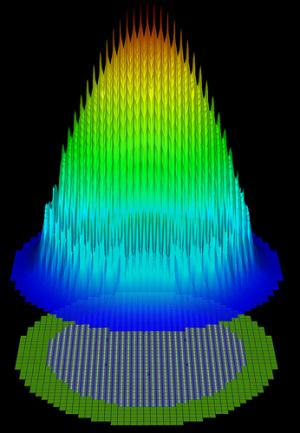
\includegraphics[height=1.75in,clip]{UNIC_powerDist}
    \end{figure}
  \end{column}
\end{columns}
\end{frame}

%%%%%%%%%%%%%%%%%%%%%%%%%%%%%%%%%%%%%%%%%%%%%%%%%%%%%%
%%%%%%%%%%%%%%%%%%%%%%%%%%%%%%%%%%%%%%%%%%%%%%%%%%%%%%
\begin{frame}{Categories}
\underline{Experiment}: Experimental scientists work by \alert{observing how} nature behaves\\
\vspace*{0.25 in}
\underline{Theory}: Theoretical scientists use the language of mathematics to \alert{explain and predict} the behavior of nature\\
\vspace*{0.25 in}
\underline{Computation}: Computational scientists use theoretical and experimental knowledge to \alert{create computer-based models} of aspects of nature
\end{frame}

%%%%%%%%%%%%%%%%%%%%%%%%%%%%%%%%%%%%%%%%%%%%%%%%%%%%%%
%%%%%%%%%%%%%%%%%%%%%%%%%%%%%%%%%%%%%%%%%%%%%%%%%%%%%%
\begin{frame}{Computational Science/Engineering}
\textcolor{dgreen}{Computational Science} seeks to gain understanding principally through the analysis of mathematical models on high performance computers.\\
\vspace*{0.25 in}
The term \textcolor{dgreen}{computational scientists} has been coined to describe scientists, engineers, and mathematicians who apply high performance computer technology in innovative and essential ways to advance the state of knowledge in their respective disciplines.\\
\vspace*{0.25 in}
Thus, we distinguish it from \textcolor{dgreen}{computer science}, which is the study of \emph{computer and computation} and \emph{theory and experiment}, the traditional form of science. 
\end{frame}

%%%%%%%%%%%%%%%%%%%%%%%%%%%%%%%%%%%%%%%%%%%%%%%%%%%%%%
%%%%%%%%%%%%%%%%%%%%%%%%%%%%%%%%%%%%%%%%%%%%%%%%%%%%%%
%\begin{frame}{The Hacker Within}
%Learn/teach skills to be a successful computational scientist
%\begin{itemize}
%\item Brand new chapter at Berkeley
%\item Wednesdays, 4-6 pm, 2nd floor of Chase Building (by the BART)
%\item Will teach skills useful for this course
%\item Valuable resource; lots of fun
%\item Website: http://thehackerwithin.github.io/berkeley/
%\item GitHub: https://github.com/thehackerwithin/berkeley
%\item in the news: http://www.news.wisc.edu/19236
%\end{itemize}
%\end{frame}

%%%%%%%%%%%%%%%%%%%%%%%%%%%%%%%%%%%%%%%%%%%%%%%%%%%%%%
%%%%%%%%%%%%%%%%%%%%%%%%%%%%%%%%%%%%%%%%%%%%%%%%%%%%%%
\begin{frame}{Solving Problems}
\begin{enumerate}
\item Identify the problem
\item Pose the problem in terms of a mathematical model
\item Identify a computational method for solving the model
\item Implement the computational method on a computer
\item Assess the answer in the context of the
\begin{itemize}
\item Implementation (computer language and architecture)
\item Method (discrete or continuous)
\item Model (symbolic or numerical)
\end{itemize}
Using
\begin{itemize}
\item Visualization and interpretation
\item Experimental comparisons
\item Analytical comparisons
\item Engineering judgement
\end{itemize}
\end{enumerate}
\end{frame}

%%%%%%%%%%%%%%%%%%%%%%%%%%%%%%%%%%%%%%%%%%%%%%%%%%%%%%
%%%%%%%%%%%%%%%%%%%%%%%%%%%%%%%%%%%%%%%%%%%%%%%%%%%%%%
\begin{frame}{Big Challenges}
\begin{itemize}
\item Science
\begin{itemize}
\item Global climate modeling
\item Astrophysical modeling
\item Biology: genomics; protein folding; drug design
\item \alert{Computational Material Sciences} and Nano-sciences
\end{itemize}
\item Engineering
\begin{itemize}
\item Semiconductor design
\item Earthquake and structural modeling
\item \alert{Computational fluid dynamics} 
%\item Combustion (engine design)
\item Analysis and design of \alert{nuclear reactors}
\end{itemize}
\item Business
\begin{itemize}
\item Financial and economic modeling
\item Transaction processing, web services and search engines
\end{itemize}
\item Defense
\begin{itemize}
\item Nuclear weapons -- test by simulations
\item Cryptography
\end{itemize}
\end{itemize}
\end{frame}

%%%%%%%%%%%%%%%%%%%%%%%%%%%%%%%%%%%%%%%%%%%%%%%%%%%%%%
%%%%%%%%%%%%%%%%%%%%%%%%%%%%%%%%%%%%%%%%%%%%%%%%%%%%%%
%\begin{frame}{Big Potential}
%\begin{itemize}
%\item ``Periods of rapid advancements in the sciences have often been sparked by timely technology breakthroughs in experimental technique." \vspace*{1 em}
%\item ``The next epochal period of scientific growth may be unleashed by major design breakthroughs in computer architectures and advances in modeling approaches, where supercomputers become the laboratories to test and advance new theories for which no practical experimental apparatus can be built." (1990)
%%\item Why the 90s? What's the history of computers?
%\end{itemize}
%\end{frame}

%%%%%%%%%%%%%%%%%%%%%%%%%%%%%%%%%%%%%%%%%%%%%%%%%%%%%%
%%%%%%%%%%%%%%%%%%%%%%%%%%%%%%%%%%%%%%%%%%%%%%%%%%%%%%
%\begin{frame}{Big Resources?}
%\begin{itemize}
%\item ``I think there is a world market for maybe five computers."\\
%\hspace*{0.5 in}Thomas Watson, chairman of IBM, 1943
%\item ``There is no reason for any individual to have a computer in their home."\\
%\hspace*{0.5 in}Ken Olson, president and founder of \\
%\hspace*{0.5 in}Digital Equipment Corporation, 1977
%\item ``640K [of memory] ought to be enough for anybody."\\
%\hspace*{0.5 in}Bill Gates, chairman of Microsoft, 1981
%\vspace*{0.25 in}
%\item ``Reaching a teraflop is the single biggest computer science achievement in two decades. Ten years ago, the most credible leaders in computing said it was not possible."\\
%\hspace*{0.5 in}Gil Weigand, supercomputing guru, 1996
%\end{itemize}
%\end{frame}

%%%%%%%%%%%%%%%%%%%%%%%%%%%%%%%%%%%%%%%%%%%%%%%%%%%%%%
%%%%%%%%%%%%%%%%%%%%%%%%%%%%%%%%%%%%%%%%%%%%%%%%%%%%%%
\begin{frame}{What are we trying to accomplish?}
\begin{itemize}
\item The challenge of designing a nuclear reactor is to make it as \textbf{economical} as possible while ensuring its \textbf{safety}. \vspace*{1 em}
\item This is not an easy task! \vspace*{1 em}
\item The principle of a nuclear reactor is relatively simple:
\begin{itemize}
\item \underline{Fission} creates heat within the nuclear fuel,
\item The \underline{heat} is conducted to the fuel cladding surface and to the coolant,
\item The heat is subsequently transported by a coolant through heat exchangers and ultimately to a \underline{steam} conversion plant.
\end{itemize}
\end{itemize}
\end{frame}

%%%%%%%%%%%%%%%%%%%%%%%%%%%%%%%%%%%%%%%%%%%%%%%%%%%%%%
%%%%%%%%%%%%%%%%%%%%%%%%%%%%%%%%%%%%%%%%%%%%%%%%%%%%%%
\begin{frame}{Easy?}
 \begin{figure}
   \begin{center}
     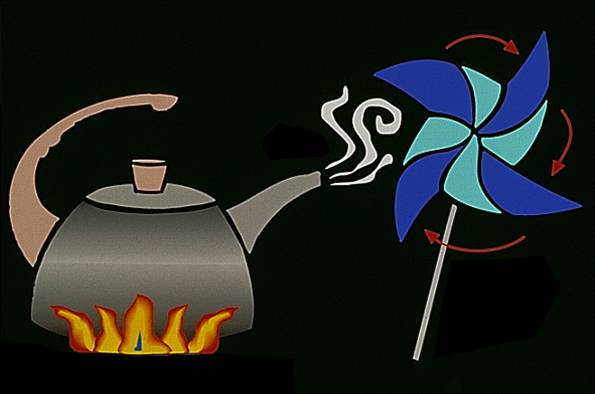
\includegraphics[height=2.5in,clip]{TeaPot}
   \end{center}
 \end{figure}
\end{frame}

%%%%%%%%%%%%%%%%%%%%%%%%%%%%%%%%%%%%%%%%%%%%%%%%%%%%%%
%%%%%%%%%%%%%%%%%%%%%%%%%%%%%%%%%%%%%%%%%%%%%%%%%%%%%%
\begin{frame}{What are we trying to accomplish?}
\begin{itemize}
\item In order to design economical and safe reactors, one must choose among a vast range of competing designs:
\begin{itemize}
\item What are the \alert{best} fuels, structure, and coolant materials; what are their appropriate ratios?
\item How does the reactor respond to component failures?
\item How does one balance those choices given competing goals of performance, lifetime, safety, and capital cost? \vspace*{1 em}
\end{itemize}
\item Ideally, one would like to base these choices on theory rather than experimental trial and error \vspace*{1 em}
\item This is where \textcolor{dgreen}{computational science} fits in...
\end{itemize}
\end{frame}

%%%%%%%%%%%%%%%%%%%%%%%%%%%%%%%%%%%%%%%%%%%%%%%%%%%%%%
%%%%%%%%%%%%%%%%%%%%%%%%%%%%%%%%%%%%%%%%%%%%%%%%%%%%%%
\begin{frame}{Early Days}
Before much computer use (e.g., 1943), things took a long time
\begin{tabu}{|X | l|}
\hline
Project & Est. Time \\\hline
Density distribution in difficult system & 2 weeks \\
Integral equation for absorption in Al slab & 2 weeks \\
Slowing-down length in H$_2$O \& related calcs & 3 weeks \\
Albedo problems & 1 week \\\hline
\end{tabu}
\begin{center}
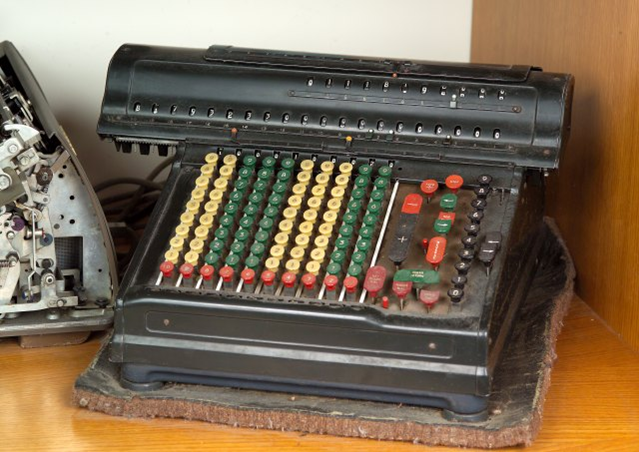
\includegraphics[height=1.5in,clip]{ACRM}
\end{center}
\end{frame}

%%%%%%%%%%%%%%%%%%%%%%%%%%%%%%%%%%%%%%%%%%%%%%%%%%%%%%
%%%%%%%%%%%%%%%%%%%%%%%%%%%%%%%%%%%%%%%%%%%%%%%%%%%%%%
\begin{frame}{Adolescence -- Early 1980s}
\begin{itemize}
\item NE was at the forefront of computer applications (!)
%pushing the envelope for ever greater computing resources and related advances in computational science.
\item Major early success story in the computational sciences:
\begin{itemize}
\item Reduced the burden of experiment
\item Contributed greatly to reactor design
\end{itemize}
\item However, modeling was severely constrained 
%Even state-of-the-art machines such as Cray-1 were 
\begin{itemize}
\item Unable to explicitly model the key physical phenomena within a reactor
\item Low-dimensional representation
\item Lumped parameter models
\item Empirical correlations with tunable parameters established largely by experiments
\end{itemize}
\end{itemize}
\end{frame}

%%%%%%%%%%%%%%%%%%%%%%%%%%%%%%%%%%%%%%%%%%%%%%%%%%%%%%
%%%%%%%%%%%%%%%%%%%%%%%%%%%%%%%%%%%%%%%%%%%%%%%%%%%%%%
\begin{frame}{Adolescence $\rightarrow$ Today's Challenges}
\begin{itemize}
\item Computing limitations caused
\begin{itemize}
\item Heavy reliance on expensive and often complicated experiments
\item Inaccuracy resulted in \emph{significant design margins} $\rightarrow$ negative impact on plant economics
\item Exploration of novel reactor design concepts was greatly constrained 
%by fundamental limitations in the predictability of the models
\vspace*{1 em}
\end{itemize}
\item Many codes developed then are still used 
\pause
\item Can we update these tools?
\pause
\item Do we need to design new tools?
\pause
\item What methods will take us into the future?
\pause
\item What will the architectures look like?
\pause
\item How do we successfully navigate that interplay?
\end{itemize}
\end{frame}

%%%%%%%%%%%%%%%%%%%%%%%%%%%%%%%%%%%%%%%%%%%%%%%%%%%%%%
%%%%%%%%%%%%%%%%%%%%%%%%%%%%%%%%%%%%%%%%%%%%%%%%%%%%%%
\begin{frame}{Current State}
2010: the DOE announced \emph{Oak Ridge National Laboratory} won the Nuclear Energy Modeling and Simulation Energy Innovation Hub (reawarded for 10 years), including:	
\begin{itemize}
\item Electric Power Research Institute (EPRI), Palo Alto, CA
\item Idaho National Laboratory, Idaho Falls, ID
\item Los Alamos National Laboratory, Los Alamos, NM
\item Massachusetts Institute of Technology, Cambridge, MA
\item North Carolina State University, Raleigh, NC
\item Sandia National Laboratories, Albuquerque, NM
\item Tennessee Valley Authority, Knoxville, TN
\item University of Michigan, Ann Arbor, MI
\item Westinghouse Electric Company, Pittsburgh, PA
\end{itemize}
\end{frame}

%%%%%%%%%%%%%%%%%%%%%%%%%%%%%%%%%%%%%%%%%%%%%%%%%%%%%%
%%%%%%%%%%%%%%%%%%%%%%%%%%%%%%%%%%%%%%%%%%%%%%%%%%%%%%
\begin{frame}{Consortium for Advanced Simulation of Light Water Reactors}
\begin{center}

\includegraphics[height=0.75in,clip]{CASL}
\end{center}
CASL was established to provide leading edge modeling and simulation (M\& S) capability to improve the performance of \textit{currently operating light water reactors}. Our vision is safer and more productive commercial nuclear power production afforded through comprehensive science-based predictive M\& S technology...CASL is developing the Virtual Environment for Reactor Applications, \textbf{VERA}. CASL's VERA software simulates nuclear reactor physical phenomena using coupled multi-physics models. 
\end{frame}


%%%%%%%%%%%%%%%%%%%%%%%%%%%%%%%%%%%%%%%%%%%%%%%%%%%%%%
%%%%%%%%%%%%%%%%%%%%%%%%%%%%%%%%%%%%%%%%%%%%%%%%%%%%%%
\begin{frame}{MOOSE and SHARP}
\begin{center}
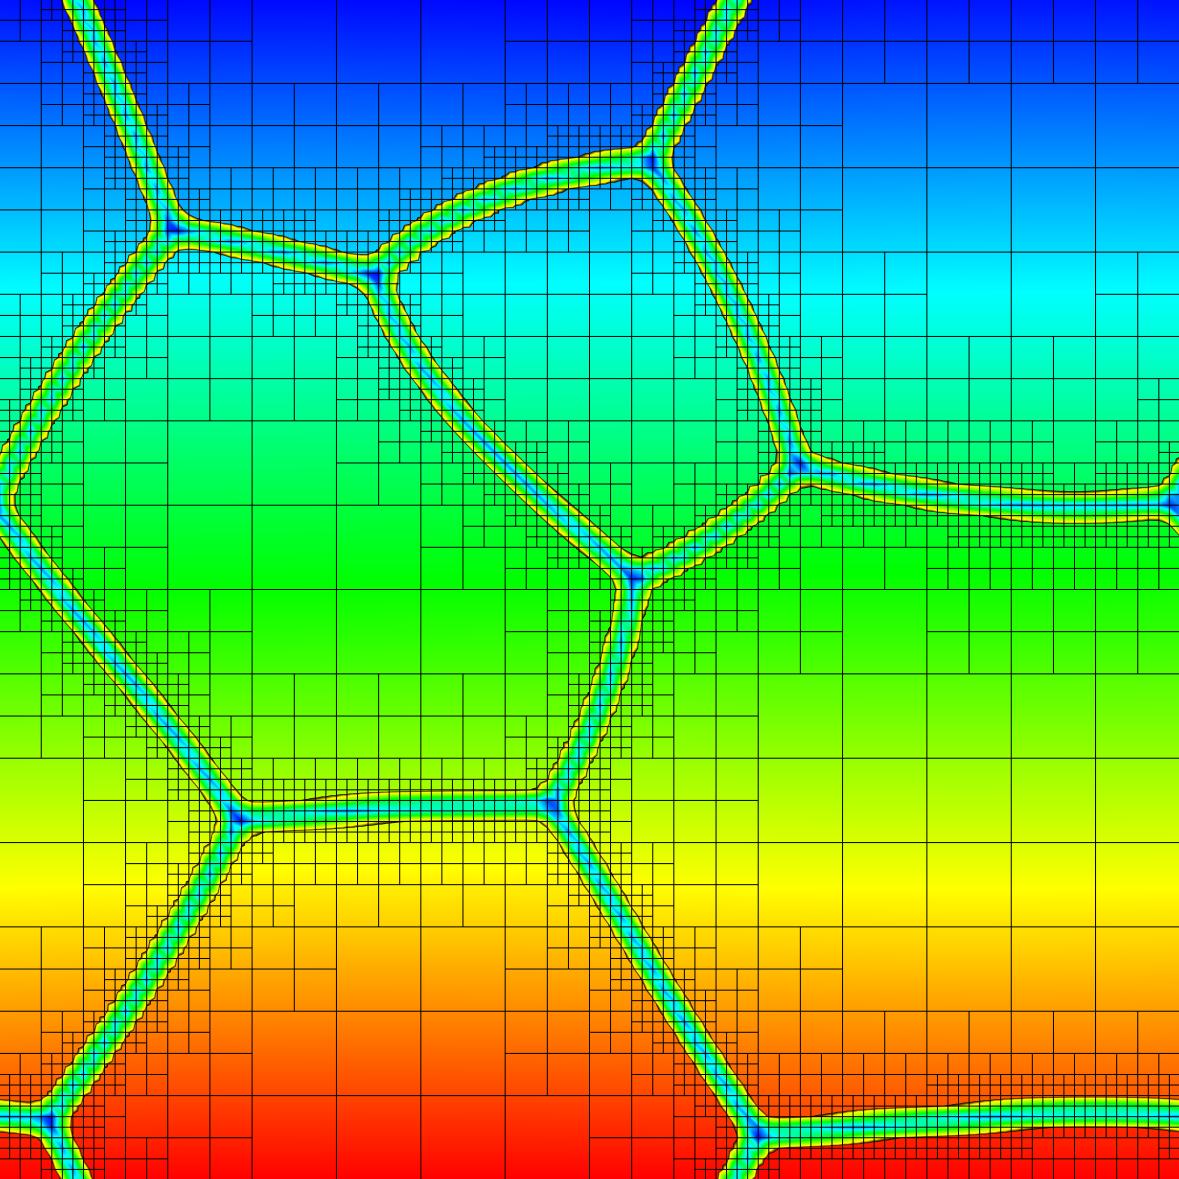
\includegraphics[height=0.75in,clip]{moose}
\end{center}
\begin{itemize}
\item \textcolor{RawSienna}{MOOSE}: The Multiphysics Object-Oriented Simulation Environment (MOOSE) is a finite-element, multiphysics framework primarily developed by Idaho National Laboratory. It provides a high-level interface to some of the most sophisticated nonlinear solver technology on the planet.
\item \textcolor{RawSienna}{SHARP}: The Simulation-based High-efficiency Advanced Reactor Prototyping (SHARP) suite of codes enables virtual design and engineering of nuclear plant behavior...researchers have developed a set of simulation tools that provide a highly detailed description of the reactor core and the nuclear plant behavior. 
\end{itemize}
\end{frame}

%%%%%%%%%%%%%%%%%%%%%%%%%%%%%%%%%%%%%%%%%%%%%%%%%%%%%%
%%%%%%%%%%%%%%%%%%%%%%%%%%%%%%%%%%%%%%%%%%%%%%%%%%%%%%
\begin{frame}{Supercomputing in Research}
These kinds of simulations require time on the fastest computers in the world
\begin{itemize}
\item \textcolor{RawSienna}{Titan} (ORNL): 299,008 Opteron Cores (CPU) + 18,688 K21 Keplers (GPU); \textcolor{dgreen}{27 petaflops}
\item \textcolor{RawSienna}{IBM Sequoia} (LLNL): 1,572,864 cores (CPU); \\\textcolor{dgreen}{16.32 petaflops}
\end{itemize}
\begin{figure}
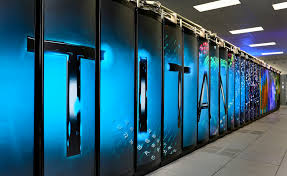
\includegraphics[height=1.1in,clip]{Titan}
\hfill
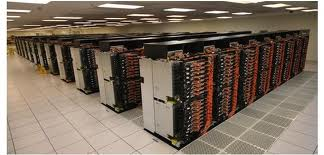
\includegraphics[height=1.1in,clip]{Sequoia}
\end{figure}
\end{frame}

%%%%%%%%%%%%%%%%%%%%%%%%%%%%%%%%%%%%%%%%%%%%%%%%%%%%%%
%%%%%%%%%%%%%%%%%%%%%%%%%%%%%%%%%%%%%%%%%%%%%%%%%%%%%%
\begin{frame}{It's Important}
``. . . At Oak Ridge National Laboratory, they're using supercomputers to get a lot more power out of our nuclear facilities . . . . "

\vspace*{0.5 in}
President Obama, 2011 State of the Union\\
\href{http://www.casl.gov/media/20110127\_news.shtml}{http://www.casl.gov/media/20110127\_news.shtml}
\end{frame}

%%%%%%%%%%%%%%%%%%%%%%%%%%%%%%%%%%%%%%%%%%%%%%%%%%%%%%
%%%%%%%%%%%%%%%%%%%%%%%%%%%%%%%%%%%%%%%%%%%%%%%%%%%%%%
\begin{frame}{What Can We Accomplish?}
\begin{itemize}
\item Predictive simulation 
\item Model entire facilities at a new level of fidelity
\item Coupled multi-physics
%Lets us reduce margins, extend existing reactor lifetimes, and consider new designs.
\end{itemize}
\begin{figure}
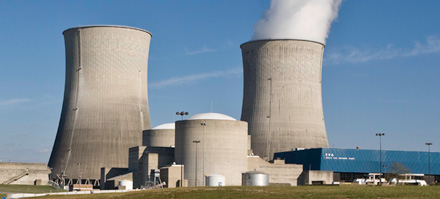
\includegraphics[height=1.2in,clip]{WattsBar}
\hfill
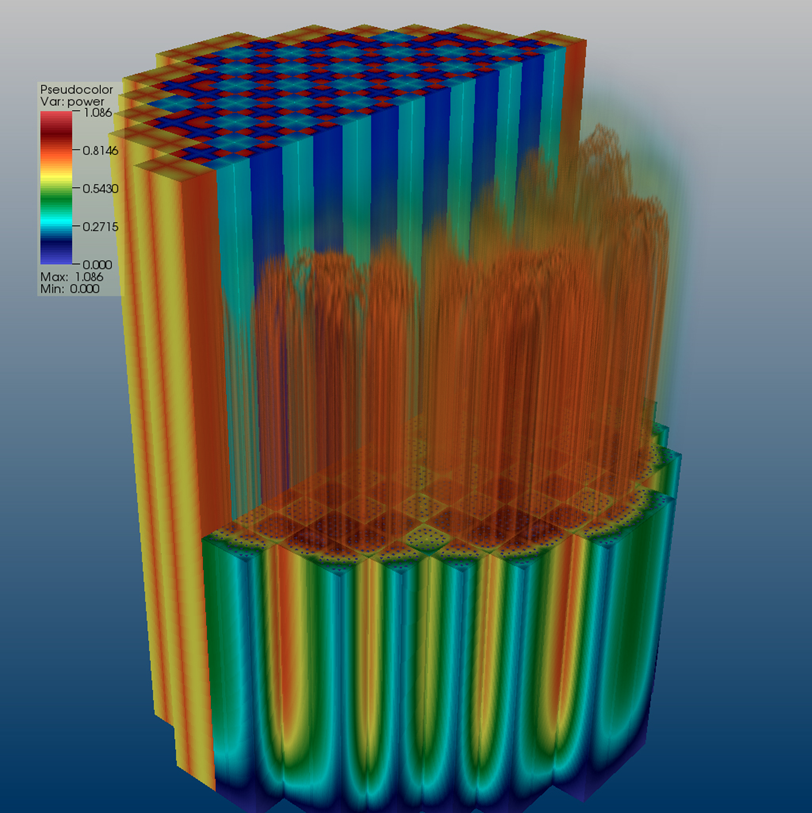
\includegraphics[height=1.2in,clip]{DenovoCore}
\end{figure}
\end{frame}

%%%%%%%%%%%%%%%%%%%%%%%%%%%%%%%%%%%%%%%%%%%%%%%%%%%%%%
%%%%%%%%%%%%%%%%%%%%%%%%%%%%%%%%%%%%%%%%%%%%%%%%%%%%%%
\begin{frame}{What Can We Accomplish?}
\underline{Integrate}
\begin{itemize}
\item existing nuclear energy and nuclear national security modeling and simulation capabilities
\item and associated expertise
\item with high-performance computing
\end{itemize}    
to solve problems that were \emph{previously unthinkable or impractical} in terms of the computing power required to address them.

\vspace*{1em}
However, these computer simulations will not completely eliminate the need for \emph{experimental or measurement data} to confirm or ``validate" the software. 

\vspace*{1em}
\hspace*{0.25 in} John Wagner, ORNL
\end{frame}

%"Traditionally, reactor models for radiation dose assessments have considered just the reactor core, or a small part of the core," Wagner says. "However, we're now simulating entire nuclear facilities, such as a nuclear power reactor facility with its auxiliary buildings and the ITER fusion reactor, with much greater accuracy than any other organization that we're aware of." 
%
%More accurate models enable nuclear plants to be designed with more accurate safety margins and shielding requirements, which helps to improve safety and reduce costs. The technology that makes this sort of leading-edge simulation possible is a combination of ORNL's Jaguar, the world's fastest supercomputer; advanced transport methods; and a next-generation software package called Denovo.
%
%DENOVO is a Scalable HPC Transport Code for Multi-Scale Nuclear Energy Applications
%http://computing.ornl.gov/SC09/videos/tomevans_1Mb.mov

%%%%%%%%%%%%%%%%%%%%%%%%%%%%%%%%%%%%%%%%%%%%%%%%%%%%%%
%%%%%%%%%%%%%%%%%%%%%%%%%%%%%%%%%%%%%%%%%%%%%%%%%%%%%%
\begin{frame}{Are You Up To the Challenge?}
\begin{figure}

\includegraphics[height=2.5in,clip]{science}
\end{figure}
\end{frame}

\end{document}
